%%%% Small single column format, used for CIE, CSUR, DTRAP, JACM, JDIQ, JEA, JERIC, JETC, PACMCGIT, TAAS, TACCESS, TACO, TALG, TALLIP (formerly TALIP), TCPS, TDSCI, TEAC, TECS, THRI, TIIS, TIOT, TISSEC, TIST, TKDD, TMIS, TOCE, TOCHI, TOCL, TOCS, TOCT, TODAES, TODS, TOIS, TOIT, TOMACS, TOMM (formerly TOMCCAP), TOMPECS, TOMS, TOPC, TOPLAS, TOPS, TOS, TOSEM, TOSN, TRETS, TSAS, TSC, TSLP, TWEB.
% \documentclass[acmsmall]{acmart}

%%%% Large single column format, used for IMWUT, JOCCH, PACMPL, POMACS, TAP, PACMHCI
% \documentclass[acmlarge,screen]{acmart}

%%%% Large double column format, used for TOG
% \documentclass[acmtog, authorversion]{acmart}

%%%% Generic manuscript mode
\documentclass[manuscript, review = false, screen]{acmart}

\usepackage[utf8]{inputenc} 
\usepackage{soul}
\usepackage{xcolor}
\usepackage{subcaption}
\usepackage{todonotes}

%
% defining the \BibTeX command - from Oren Patashnik's original BibTeX documentation.
\def\BibTeX{{\rm B\kern-.05em{\sc i\kern-.025em b}\kern-.08emT\kern-.1667em\lower.7ex\hbox{E}\kern-.125emX}}

% Rights management information.
% This information is sent to you when you complete the rights form.
% These commands have SAMPLE values in them; it is your responsibility as an author to replace
% the commands and values with those provided to you when you complete the rights form.
%
% These commands are for a PROCEEDINGS abstract or paper.
%\copyrightyear{2018}
%\acmYear{2018}
%\setcopyright{acmlicensed}
%\acmConference[Woodstock '18]{Woodstock '18: ACM Symposium on Neural Gaze Detection}{June 03--05, 2018}{Woodstock, NY}
%\acmBooktitle{Woodstock '18: ACM Symposium on Neural Gaze Detection, June 03--05, 2018, Woodstock, NY}
%\acmPrice{15.00}
%\acmDOI{10.1145/1122445.1122456}
%\acmISBN{978-1-4503-9999-9/18/06}

%
% These commands are for a JOURNAL article.
%\setcopyright{acmcopyright}
%\acmJournal{TSC}
%\acmYear{2018}\acmVolume{37}\acmNumber{4}\acmA%rticle{111}\acmMonth{8}
%\acmDOI{10.1145/1122445.1122456}

%
% Submission ID.
% Use this when submitting an article to a sponsored event. You'll receive a unique submission ID from the organizers
% of the event, and this ID should be used as the parameter to this command.
%\acmSubmissionID{123-A56-BU3}

%
% The majority of ACM publications use numbered citations and references. If you are preparing content for an event
% sponsored by ACM SIGGRAPH, you must use the "author year" style of citations and references. Uncommenting
% the next command will enable that style.
%\citestyle{acmauthoryear}

%
% end of the preamble, start of the body of the document source.
\begin{document}
%
% The "title" command has an optional parameter, allowing the author to define a "short title" to be used in page headers.

\title[Augmented Virtual Reality Meditation: Shared Dyadic Biofeedback Increases Social Presence Via Respiratory Synchrony]{Augmented Virtual Reality Meditation: Shared Dyadic Biofeedback Increases Social Presence Via Respiratory Synchrony}



%
% The "author" command and its associated commands are used to define the authors and their affiliations.
% Of note is the shared affiliation of the first two authors, and the "authornote" and "authornotemark" commands
% used to denote shared contribution to the research.


\author{Simo Järvelä}
\affiliation{%
    \institution{University of Helsinki, }
    \institution{Tampere University, }
    \instituion{Aalto University}}
\email{simo.v.jarvela@helsinki.fi}

\author{Benjamin Cowley}
\affiliation{%
    \institution{University of Helsinki}}
\email{ben.cowley@helsinki.fi}

\author{Mikko Salminen}
\affiliation{%
    \institution{University of Tampere}}
\email{mikko.salminen@tuni.fi}    

\author{Giulio Jacucci}
\affiliation{%
    \institution{University of Helsinki}}
\email{giulio.jacucci@helsinki.fi}

\author{Juho Hamari}
\affiliation{%
    \institution{University of Tampere}}
\email{juho.hamari@tuni.fi}


\author{Niklas Ravaja}
\affiliation{%
    \institution{University of Helsinki}}
\email{niklas.ravaja@helsinki.fi}





%
% By default, the full list of authors will be used in the page headers. Often, this list is too long, and will overlap
% other information printed in the page headers. This command allows the author to define a more concise list
% of authors' names for this purpose.
\renewcommand{\shortauthors}{Järvelä, et al.}

%
% The abstract is a short summary of the work to be presented in the article.

\begin{abstract}
In a novel experimental setting, we augmented a variation of traditional compassion meditation with our custom built VR environment for multiple concurrent users. The presence of another user's avatar in shared virtual space supports social interactions and provides an active target for evoked compassion. The system incorporates respiration and brainwave -based biofeedback to enable closed-loop interaction of users based on their shared physiological state. Specifically, we enhanced interoception and the deep empathetic processes involved in compassion meditation with real time visualizations of: breathing rate, level of approach motivation assessed from EEG frontal asymmetry, and dyadic synchrony of those signals between two users. We manipulated these interventions across eight separate conditions (dyadic or solo meditation; brainwave, breathing, both or no biofeedback) in an experiment with 39 dyads (N=78), observing the effect of conditions on self-reported experience and physiological synchrony. We found that each different shared biofeedback type increased users' self-reported empathy and social presence, compared to no-biofeedback or solo conditions. Our study illustrates how dyadic synchrony biofeedback can expand the possibilities of biofeedback in affective computing and VR solutions for health and wellness.
\end{abstract}



%
% The code below is generated by the tool at http://dl.acm.org/ccs.cfm.
% Please copy and paste the code instead of the example below.
%

%
% Keywords. The author(s) should pick words that accurately describe the work being
% presented. Separate the keywords with commas.

\keywords{VR, empathy, meditation, neurofeedback, psychophysiology}

%
% A "teaser" image appears between the author and affiliation information and the body
% of the document, and typically spans the page.
\begin{teaserfigure}
  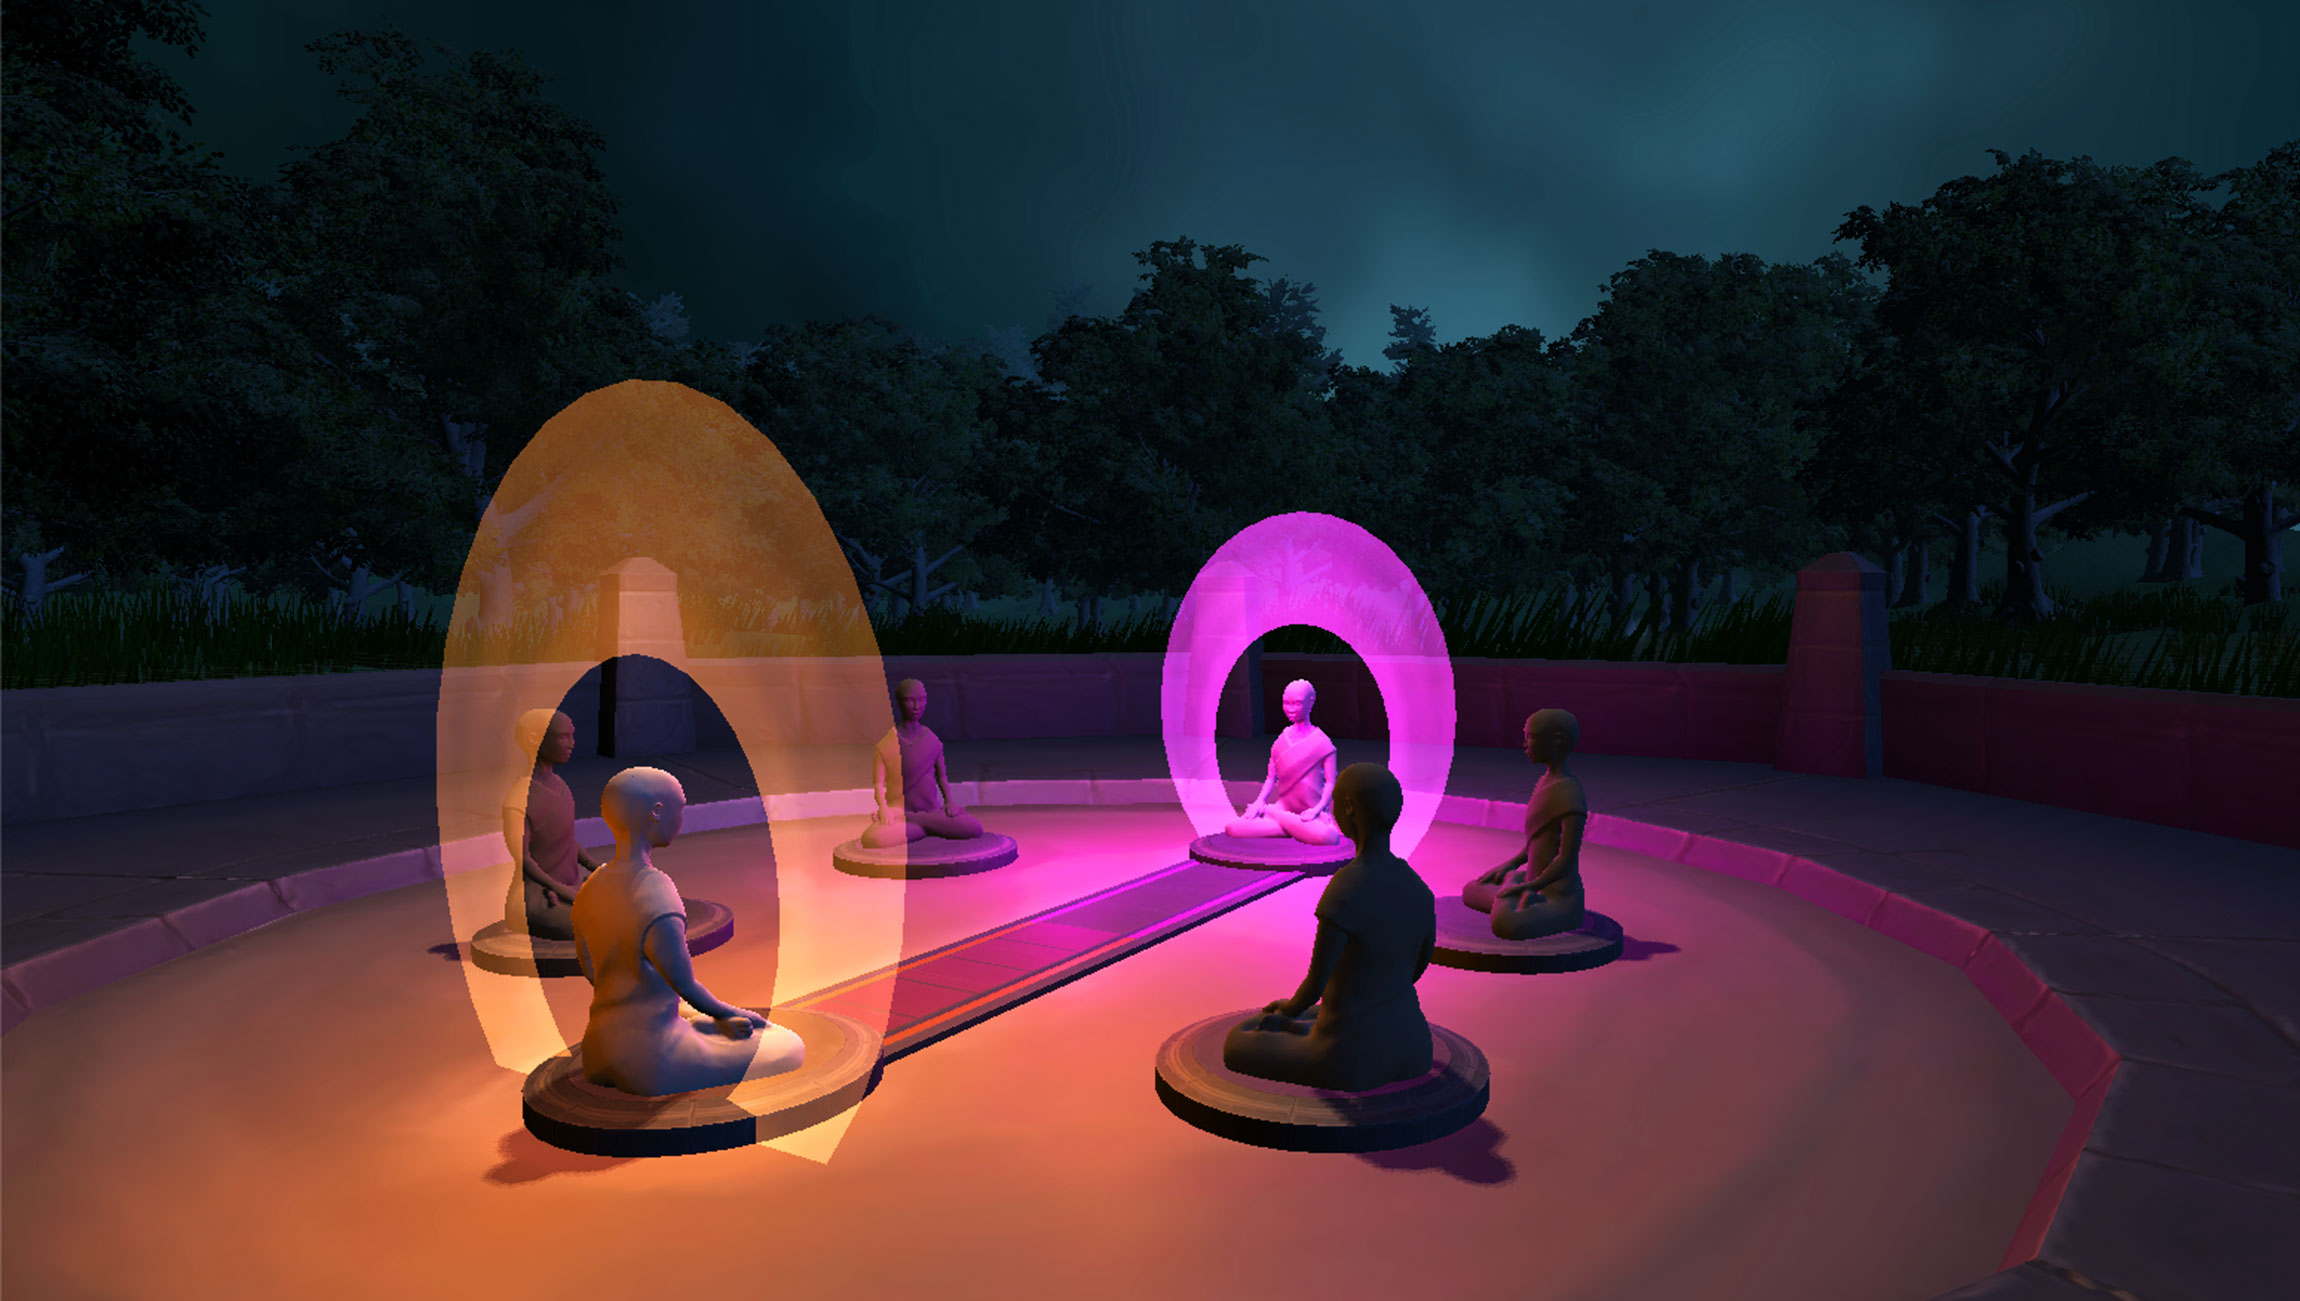
\includegraphics[width=\textwidth]{images/DYNECOM_All_large.jpg}
  \caption{Overview of the scene elements and dyadic visualizations.}
  \Description{Overview of the scene elements and dyadic visualizations.}
  \label{fig:teaser}
\end{teaserfigure}

%
% This command processes the author and affiliation and title information and builds
% the first part of the formatted document.
\maketitle

\section{Introduction}
Recent years have seen the rapid development of virtual reality (VR) environments and related technology, which have also been utilized as tools for improving personal well-being, for example as a platform for mindfulness-based meditation practice \cite{Shaw2007,Gromala2015,Kosunen2016}. A strong presence-inducing and disturbance-free virtual environment \cite{Coelho2006,Schuemie2004,Welch1996} seems an ideal solution for quick stress management exercises during the work day, where longer breaks and separate physical spaces would be impractical. In this paper, we present an approach to extend that basic idea in two ways: firstly, by incorporating respiration and brain wave -based neurofeedback and visualizations to support meditation, and secondly, by enabling social interaction in a multi-user virtual space where more than one user can meditate simultaneously in VR. Additionally, we present how these two advances can be tied together by measuring and visualizing dyadic physiological synchrony --- i.e. the joint changes in physiological signals ---  between users, enabling a system responsive to the shared physiological states of the users. Augmenting a variation of traditional compassion meditation with our VR system DYNECOM, we conducted a controlled laboratory experiment to examine how the different neurofeedback types affected both the amount of physiological synchrony between the users of the shared space and their self-reported empathy and social presence.


\section{Theoretical background}
\subsection{VR, meditation, and biofeedback}
In general, meditation exercises include various practices and traditions that are often ``\textit{complex emotional and attentional regulatory strategies developed for various ends, including the cultivation of well-being and emotional balance}'' \cite{Lutz2008a}. The positive effects of various meditation practices include, for example, the treatment for insomnia \cite{Woolfolk1976} and headache \cite{BENSON1974}, reduced blood serum cortisol levels, and reduced systolic and diastolic pressure and pulse rate \cite{Sudsuang1991}. Long term meditation has also been shown to lead to changes in the attention-related brain areas \cite{Chiesa2010}. Mindfulness-related compassion and loving-kindness meditation styles have been found to increase social connectedness, positive affect, and empathy \cite{Hutcherson2008,Hofmann2011}.

Meditation has traditionally involved a dedicated physical space: however, having a dedicated clear space for meditation, especially during work hours in the office environment, is quite challenging. This difficulty is compounded if we consider group or pair-wise meditation. With the popularization of VR devices and the current rise of interest in mindfulness and similar activities, the combination of VR and meditation feels like a natural coupling to address this issue, and a simple VR solution can provide that personal distraction-free moment necessary for mindfulness. Multi-user VR also enables sharing of the meditation space with others far more easily and over physical distances for group meditation purposes. These pragmatic benefits of VR meditation have the potential to considerably lower the threshold of practicing meditation in our everyday lives. There are already various VR implementations of guided meditation and relaxation protocols. For example, in Relaxation Island \cite{Waterworth2004} the user can walk in a soothing environment using a seashell shaped joystick for navigation; initial results indicated that the use of the system had a relaxing effect, as intended. 

Biofeedback is a closed-loop interactive system presenting measured physiological signals back to the user through real-time audiovisual, haptic, or other stimulation. It has been increasingly utilized in augmented meditation, such as in \citet{Chittaro2014, CarissoliClaudia2015}. Typically such systems utilize cardiac measures, electrodermal activity, or occasionally brain wave measures, that could provide information regarding arousal and stress levels of the user \cite{cacioppo2007handbook}. Biofeedback has been utilized in a therapeutic context for several decades, and it has been suggested \cite{calderon2004biofeedback} that its effects have three stages 1) awareness 2) learning 3) transfer. In the first stage a person becomes aware of bodily states highlighted by the biofeedback through interoceptive awareness \cite{Craig2002,dunn2010listening}; in the second stage the biofeedback helps the person to learn control over these bodily states; and finally in the third stage what has been learned is transferred to other contexts outside the immediate biofeedback setting. Which learning paradigm to use in any given setting, and what neurophysiological mechanisms occur for each type of feedback and paradigm, are still under scientific inquiry. Therefore it is not a simple task to develop an evidence-based system to achieve a specific effect and learning outcome. Here, we take the view that it is not necessary to target learning or transfer outcomes (stages 2 and 3); rather, it is sufficient to induce heightened self-awareness (stage 1) by just guiding attention to certain bodily dynamics. In addition to interoceptive awareness, biofeedback can also be utilized when shared among users, to provide socially relevant emotional information. Our system thus aims to use biofeedback to affect users' social and affective processes, without aiming at any long-term learning effects.

Biofeedback functionality has been utilized in some VR applications already. For example, Virtual Meditative Walk \cite{Gromala2015} teaches chronic pain patients a mindfulness-based stress reduction technique, utilizing sound effects, immersive VR environment, and biofeedback using galvanic skin response (GSR) to control the weather conditions in the environment. In Meditation Chamber \cite{Shaw2007}, in addition to the GSR, breathing rate and blood volume pulse were utilized to control features of the environment. Also, the information from brain electrical activation, obtained by the electroencephalography (EEG), can be used in generating feedback. EEG is a relevant method for studying meditation, given that different cognitive and conscious states are related to respective neurophysiological states. Previous studies have shown that the electrical activation of the brain can be studied as the powers of various frequency bands, that are related to, for example, cognitive and affective processes \cite{Aftanas2001,Klimesch1998,Klimesch1999}. The frontal asymmetry (FA) of the {\it alpha} frequency band (8-13 Hz), quantified as a relative difference between activations of the anterior left and right regions, is one of the most widely used psychophysiological indices in empathy research. The frontal left and right regions are parts of two separate neural systems that are related to approach and withdrawal motivations, respectively \cite{Klimesch1998,Klimesch1999}. Interestingly, the experience of empathy and (separately) the ability to empathize are related to increased left frontal activation \cite{Field2009,HarmonJones2003,JONES2009}. Thus, by measuring electrical brain activation from the scalp with EEG and calculating frontal asymmetry, we can assess withdraw/approach motivation that is closely linked to empathy. This gives us a responsive real-time measure of empathy that is not dependent on self-reporting (with its attendant reporting biases), and furthermore, the continuous signal can be utilized in biofeedback in a VR system.% Without an online measurement with EEG, a biofeedback system targeting empathy is not possible until new ways to measure neurophysiological indices of empathy emerge.

While many other biosignals have been utilized in biofeedback, a limited number of systems utilizing neurofeedback exist, e.g. \cite{Hinterberger2011,Sas}. One of these is the recent neuroadaptive VR environment RelaWorld, designed to train attention skills and also for relaxation \cite{Kosunen2017,Kosunen2016}. The feedback took the form of a levitation effect and increased opaqueness or fog in the environment (a tranquil shore view), and was adaptive to the user's EEG alpha (8-13 Hz) and theta (4-6 Hz) frequency band changes. In previous studies, these frequency band activations have been related to relaxedness and focused attention, respectively. Initial results implied that the neurofeedback functionality increased the self-reported sense of presence and EEG theta band power.

\subsection{Supporting empathic interactions in shared VR meditation}
Like RelaWorld, DYNECOM incorporates EEG-based neurofeedback but adds social dynamics to the environment by having multiple simultaneous users sharing the same VR space. This novel combination of features opens up the possibility to augment primal social processes in VR by providing social information \cite{Van_Kleef_2010} to users of the shared VR space. Meditation is primarily a solitary endeavor: even in group meditation settings where a physical space is shared, the meditation activity itself is primarily a personal effort. However, the various forms of loving-kindness and compassion meditation, while typically exercised alone, can be seen at least as somewhat social as they strongly focus on empathic feelings towards others. A natural extension of this is to have the target of the compassion meditation present. In the VR the presence of another user is represented with an avatar. Cognitively, many aspects of traditional compassion meditation seem to involve empathy-related processes \cite{Hutcherson2008, Hofmann2011}. The system aims to induce primarily first-stage biofeedback effects: increasing users' awareness of shared bio-dynamics and providing socially usable information, thereby augmenting the VR to support empathy and social presence. To a lesser extent, DYNECOM should support users' own interoception.% The system does not as such aim at specific learning outcomes, but to support the activity conducted within the shared VR, and leave the positive learning outcomes to the meditation activity itself.

No single definitive consensus on the definition of empathy exists. In fact, there are numerous frameworks and definitions highlighting different perspectives to or components of empathy \cite{Cuff_Brown_Taylor_Howat_2016}. One aspect of empathy is cognitive empathy, or empathic accuracy: the ability to recognize emotional states of others \cite{Janssen_2012}. Another aspect of empathy is the merging of the feelings with someone, while sympathy can be defined as an awareness of the other's feelings but not experiencing those same feelings \cite{Escalas2003}. The spontaneous mimicry of the empathized other may, via emotional contagion, build the subjective feeling of empathy and thus emotional resonance \cite{Hofelich2011, Oberman2007}. Previous studies have related empathy to various positive outcomes, for example, to increased willingness to help \cite{Coke1978}. Social presence \cite{Biocca_Harms_2002, Biocca_Harms_Burgoon_2003, Harms_Biocca_2004} is another theoretical construct closely related to empathy. \citet{Harms_Biocca_2004} defined it as follows: ``\textit{Social presence  in  a  mutual  interaction  with  a  perceived  entity  refers  to  the  degree  of  initial  awareness,  allocated  attention,  the  capacity  for  both  content  and  affective  comprehension,  and  the  capacity  for  both affective and behavioral interdependence with said entity.}'' Of these various components of social presence, particularly affective understanding and affective interdependence could be seen as parts of empathy-related processing.

\textcolor{blue}{This leads us to the first research question: {\bf how are empathy and social presence affected by neurofeedback training with a partner in a VR meditation environment}?} To study this, we looked at the effect of including a rarely-studied form of biofeedback --- dyadic physiological-synchrony feedback --- in a shared VR meditation session. 

Physiological synchrony refers to the extent to which physiological signals of two or more people are associated with each other, such as a mutual increase in heart rate (HR) during a shared experience \cite{Palumbo_Marraccini_Weyandt_Wilder-Smith_McGee_Liu_Goodwin_2016}. Such indices can be calculated from physiological measurement data when they have been recorded from two or more persons simultaneously. While the idea of dyadic synchrony is not a new one, it has not been well-studied in a meditation context, and psychological phenomena related to it remain largely unmapped. In a number of previous studies, the synchronization of physiological activities between two persons has been related to empathy. For example, synchronization of the electrodermal activation (EDA, sweating of the hands) between a therapist and a patient was related to the patient's perception of the therapist's empathy towards him or her, in a study by Marci et al. \cite{Marci2007}. Matching physiological states have also been related to empathic accuracy; more accurate ratings of a videotape were obtained when there was stronger physiological linkage between the rater and the person on the videotape \cite{levenson1992empathy}. In addition, social presence has been associated with physiological synchrony \cite{Jarvela_Katsyri_Ravaja_Chanel_Henttonen_2016, Ekman_Chanel_Jarvela_Kivikangas_Salminen_Ravaja_2012}. 

Dyadic neurofeedback, as used in DYNECOM, provides the users with information about how much their physiological signals are in synchrony, and consequently, information on those social and empathy-related processes that can be assessed with physiological synchrony indices. DYNECOM still provides individual-level biofeedback to support interoception, but its primary function is to support the social dynamic related to empathy. We have chosen biofeedback as a way to present socially usable information \cite{Van_Kleef_2010} to the users exploring how it can be harnessed in a social domain to augment social interactions. \textcolor{blue}{ The second research question reflects this dynamic: {\bf how does dyadic synchrony biofeedback affect physiological synchrony within dyads}?}

This approach of implementing dyadic neurofeedback in a shared VR space is, to our knowledge, completely novel. To study the effects of these VR augmentations on empathy and social presence, we developed DYNECOM VR environment and conducted a controlled laboratory experiment. Long-term effects of repeated use were not examined, only whether the forms of biofeedback and sharing the VR space with another person had significant impact on empathy, social presence, and physiological synchrony. The aim is to find ways to support empathic interactions in shared VR, to enable warmer and more compassionate social connections to be shared among computer users across the globe.



\section{System Overview}

\subsection{Hardware and setup}
The system hardware setup consists of four computers: two running the test and two for monitoring and recording. Biosignals are first recorded with Brain Products QuickAmp devices. The recording computer streams the physiological data to the network from BrainVision Recorder software in real time. Next OpenViBE \cite{OpenViBE} is run on the test computers to process the signals before sending them to the main program running through Unity3D (v2017.1.0b5)\cite{Unity3D}, where visualizations, user-end recording and networking are handled. Virtual reality is provided through two Oculus Rift headsets (2016 version) with Oculus Touch hand controllers. 3D-models were made with Blender \cite{Blender} and Adobe Photoshop \cite{Photoshop} and some assets were acquired from Unity3D asset store.

\subsection{Design of the virtual environment}
DYNECOM is built around the metaphor of ``sitting together by the campfire''. This immersive setting provides several suitable aspects: It is a relaxed social situation with a shared activity, where nature provides a relaxing background, and the built-in elements balance the wilderness with familiarity. Each session starts by showing a minimalistic room for recording the participant's baseline neurophysiological activation. It is followed by the meditation environment consisting of six stone statues sitting in a ring on a small shrine-like platform. The platform is surrounded by a short wall and a forest background lit by a cloudy evening sky. Dusk was chosen as scene lighting as a dark ambience acts as a contrasting background in the visual hierarchy, guiding attention towards the neurofeedback cues and making them easily readable.

Participants sit during the experiment and, in the virtual environment, possess one of the two statues connected by a bridge. From their perspective users see the bridge connecting to the opposite statue. To increase immersion, an audio track of pink noise resembling wind rustling through the trees was added to mask the background sound of the laboratory. Depending on the test condition, the bridge, the scene lights and the aura-like ring surrounding active statues show various visual effects or cues to inform the user of their current state. Scene layout is shown in Figure \ref{fig:teaser}.

To further guide the participants' attention, a short wall was added to encircle the platform. It acts to discourage the tendency of the users to explore the scene and limits the field of view to the essential elements. From the perspective of immersion, as the wall blocks the view down the forest the space feels enclosed, safe and more intimate. Having an open view of the sky counters possible claustrophobic anxieties, as does the low height of the wall. This conveys the idea that if needed, one could easily leave from the situation.

Compassion meditation often includes more than one target for the empathic feelings evoked during the exercise. Even though our focus is on dyadic interaction, this broader perspective was included in the design by having four passive statues sitting next to the two active ones connected by the bridge, hinting at the possibility of a group setting. 

As the study is not exploring the various effects elicited by the avatars themselves, the presentation of the participants must be extremely neutral while still being identifiable and easily approachable. Empathy towards virtual and artificial characters can be challenged by the so called uncanny valley effect, where imperfections in representation aiming for realism can cause a feeling of revulsion \cite{6213238}. As a pragmatic solution, statues are used as avatars, because they offer a target for identification without expectations of expression.

To avoid biases of inter-subjective identification, the statue is sculpted to be an androgynous and ageless humanoid lacking any strong identifiers. The face rests in a neutral relaxed expression and the statue sits cross-legged in a pose associated with mental engagement in meditative practice.

Virtual reality often causes discomfort commonly known as VR sickness. Symptoms include nausea, headache and disorientation after being exposed to virtual reality content. One potential cause for the symptoms is the disparity between perceived and real physical motion which causes conflict between sensory inputs~\cite{LaViola:2000:DCV:333329.333344}. This led us to design a static scene, further supported with visual cues suggesting embodiment in a statue.

\subsection{Affective cues and neurofeedback}
The needs of the experimental research setting placed limitations for the visual design: The measured biosignals (frontal asymmetry variance and respiration), and the synchrony between them, needed to be visually conveyed to both users via intuitive and non-distractive cues. Additionally, the activity needed to remain identical across solo and dyadic conditions.

The bridge connecting the two users acts as a display to convey biofeedback from each. It lays at a convenient viewing angle and distance, enabling the users to perceive relevant states without needing to move their head \cite{Alger2015}. A aura-like ring shape surrounds the active statues acting as an additional display for the state of the opposite participant.

Respiration is visualized with movement. The aura ring expands and contracts by the stages of breathing and a wave effect consisting of lighted bars is shown on top of the bridge. This wave effect consists of five consecutive bars that are illuminated with a fade-in effect based on exhaling intervals. When an exhalation is detected the bar effect is launched by illuminating each of the layers one at a time, starting from the one closest to the user. After a short period of time the layers withdraw and fade out back to invisible if a new exhalation is not detected. In the dyadic condition when participants breathe at the same pace, the bars colliding in the middle of the bridge flash with a bright highlight indicating the synchrony of respiration. The respiration bars and synchronous flash effects are seen in Figure \ref{fig:breathingbar}. The idea behind the respiration bar visualization was to provide rapid responsiveness of the effect to the sensor values, reminiscent of a graphic equalizer.

\begin{figure}
\begin{subfigure}{0.45\textwidth}
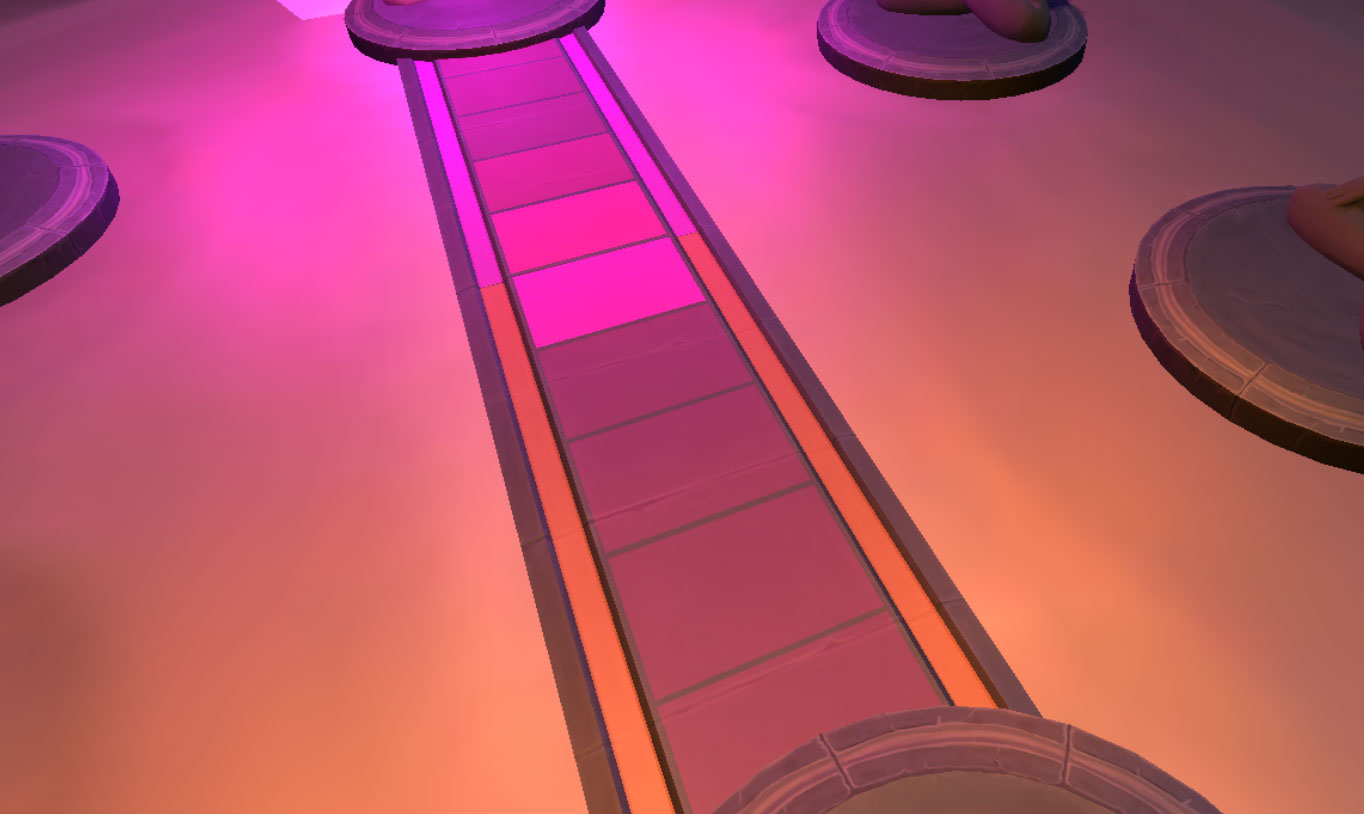
\includegraphics[width=0.99\linewidth, height=4cm]{images/DYNECOM_BarSync.jpg}
\caption{ }
\label{fig:breathingbar}
\end{subfigure}
\begin{subfigure}{0.45\textwidth}
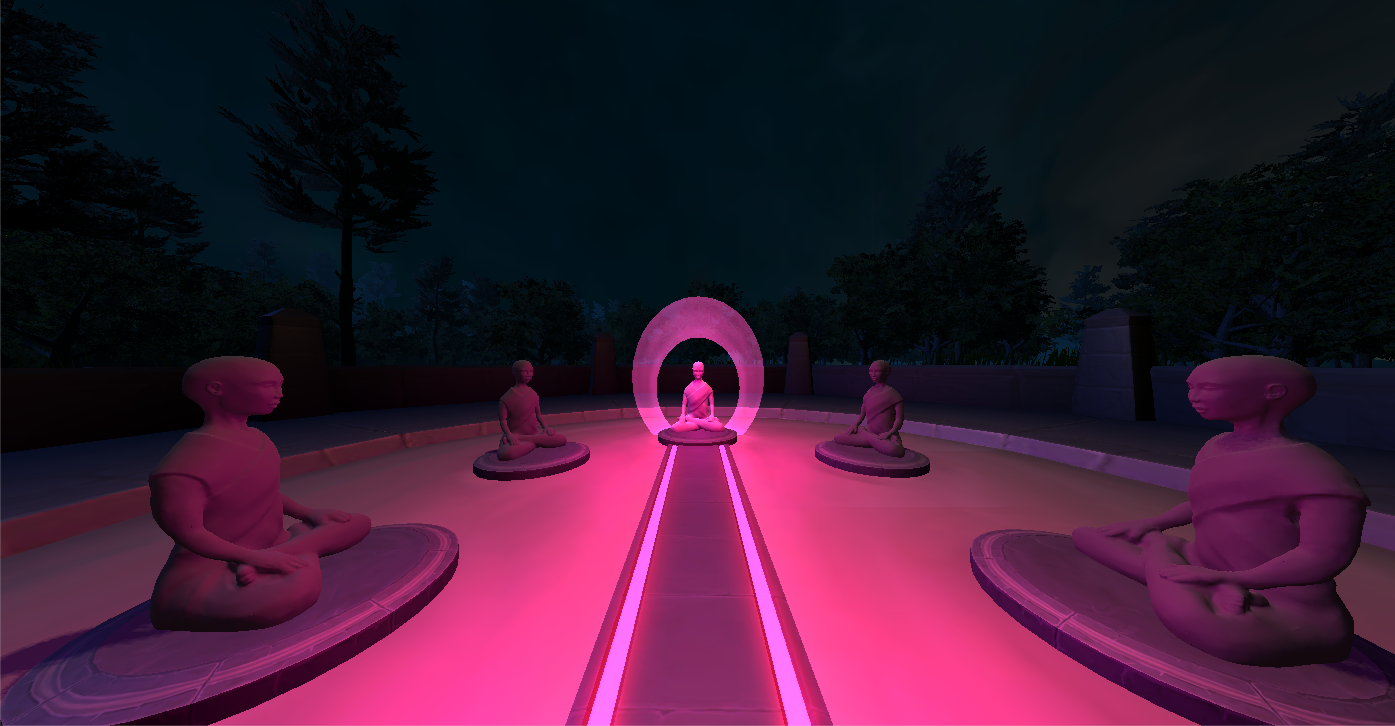
\includegraphics[width=0.99\linewidth, height=4cm]{images/glow.png}
\caption{ }
\label{fig:glow}
\end{subfigure}
\caption{Visual cues displaying both adaptations. (a) Breathing bar blink effect visualizing synchronous respiration. (b) Glow cue in the bridge recesses for a synchronous EEG-state.}
\label{fig:adaptations}
\end{figure}


In the environment different colors are used to represent the amount of empathy related approach motivation measured with the EEG. In other words, frontal asymmetry values are color encoded which acts as a visual cue for the current state of the user and their progress in meditation. Colors are present in all of the lights in the scene: the auras around the statues, the bridge side recesses, and in the breathing bars on the bridge. Colors vary in a gradient from cold green through yellow and orange to warm red and pink. Frontal asymmetry is calculated by a logarithmic formula presented by Allen et al. \cite{Allen2004}. When the measured EEG states of both users reach the limit of synchrony (within the same 1/10th of their individual current range) the glowing effect visualizing this is activated. The glowing effect raises the intensity and brightness of the color and it appears on the recesses on both sides of the bridge. Lights, aura around a statue and the glowing bridge recesses are illustrated in Figure \ref{fig:glow}. Notably, as the system highlights dyadic synchrony, it is visualized even in low approach motivation (suggesting low empathy) cases, not only in high even though higher approach motivation is expected due the meditation activity the users are conducting.

Algorithms calculating visualizations are designed to adapt to the participants throughout the subsessions. Individual minimum and maximum values of the monitored biosignals are tracked during the session and are used to define the individual's range. For frontal asymmetry, this range is then used in calculating the shown color value, using a moving average of the last 9 seconds of frontal asymmetry input. Reactivity of the algorithm was balanced through an iterative process scoping the parameters where participants felt that they could affect the visualization without it becoming too noisy. The adaptivity results in a system where users showing synchrony of color, meaning them being currently at the same respective percentage of their individual ranges at this moment in the session, even if the raw FA-values (frontal asymmetry) differ. Also, as the minimum and maximum values adapt to participant performance throughout the session, the same colors can represent different FA-values at the start and at the end of the session. Before the visualizations are engaged, a 30s monitoring is used for defining a base range for the effects. OpenViBE epoch averaging and moving averages with the range calculations are used for fault tolerance. 

Based on both feedbacks, when looking directly ahead, the lower part of the field of vision provides information supporting interoceptive awareness \cite{Craig2002, dunn2010listening}, and most of the neutral orientation focuses on information about the state of the other.

In the end, the two types of biofeedback were utilized in the DYNECOM environment are very different in nature. Firstly, EEG based frontal asymmetry is hard to manipulate consciously while respiration is very easy to control, and also to match to partner's breathing when the biofeedback provides the information. Secondly, expanding breathing aura and waves sent out when breathing are arguably more intuitive than colors changing depending on brain waves and more clearly mapped to a physiological state that is easier to self-monitor. These differences would certainly affect specific learning outcomes, if users were to spend sufficiently long periods (possibly tens of sessions over weeks) training. However, such questions are beyond the scope of our study.



\section{Experimental evaluation}
\subsection{Procedure}
The experiment was conducted on participant pairs who volunteered to the experiment together. Participants filled in a background information form before arrival. On their arrival, the participants were given a briefing with instructions regarding the operation of the virtual environment and what their task during the experiment would be, then gave written informed consent to participate. \textcolor{blue}{The participants were given written instructions what the different visualizations and color coding in the environment mean (e.g. "When the EEG adaptation is turned on, the color of the bridge and the halo around the statue will change from green (= a little) to pink (= a lot) according to how strongly you are directing the feelings you are aiming to conjure in the exercise towards the opposing statue.")} and instructed to concentrate on empathic, warm and compassionate feelings and direct them at the statue representing their pair. They were also encouraged to use the information provided by the VR environment to enhance their exercise.

Participants were seated on office chairs with wheels, allowing for minor movement, in an electrically shielded room during the experiment. The room was divided into two separate sections so there was no visual contact between the participants. EEG, electrocardiogram (ECG), EDA and respiration were measured from both participants. The experiment consisted of baseline measurement session, meditation activity, and self-reporting.

The experiment was conducted in the DYNECOM VR environment, and participants wore Oculus Rift VR-glasses for its duration. The experimental procedure took two to three hours for each pair, including the time it took to attach the neurophysiological measuring equipment and breaks in between different conditions. The duration for each pair differed due to technical aspects as well as individual differences in the time it took to fill out the questionnaires. As wearing VR-glasses can cause nausea and the experimental design's duration was rather lengthy, the participants were encouraged to take as many breaks in between subsections of the experiment as they preferred. A majority of the participants ended up taking one or two breaks, during which the VR-glasses were taken off and participants were offered water. 

\subsection{Design}
The experiment consisted of eight different conditions, each of which included a baseline measurement, meditation, and a questionnaire about the meditation experience. The baseline measurement was conducted in a VR-room with an "X" on the wall. The participants were in the baseline room until both had been there for two minutes. 

After two minutes the VR switched to the meditation environment. Condition scenarios differed based on which adaptations were being used (respiration, EEG, both, or no-biofeedback scenarios), and whether or not the other person's avatar was active in the environment (dyadic vs solo scenarios). In four solo scenarios, the avatar of the other participant was inactive; the four dyadic scenarios had the other participant's avatar active. Solo and dyadic conditions combined with four adaptation conditions: no adaptation, respiration adaptation, EEG adaptation, and respiration adaptation together with EEG adaptation. The meditation scenarios were played in the same order within each pair of participants; order was randomised across participant pairs. Each meditation session took six and a half minutes. If the adaptations were active in the scenario, the environment started adapting to the participants' neurophysiological responses after the first 30 seconds. After the meditation period, the VR switched to an interface to fill out the self-reports, which participants completed using the Oculus Touch VR hand controllers. 

\subsection{Participants}
The participants consisted of 78 volunteers (39 pairs,  32 males, 45 females, 1 other) that were recruited through student e-mail lists. The participant's age ranged between 19 and 50 years, with a mean of 26.08 years (\textit{SD} = 6.05). All participants were given two movie tickets for their participation. The participants were recruited as pairs and therefore all knew their pair before the experiment. The pairs did not involve participants who were in a romantic relationship with each other. All the participants were over 18 years old, right handed, fluent in Finnish and did not report to having any diagnosed neurological or neuropsychological disorders. All participants had completed a minimum of high school education, and 31 of them were part time or full time students at the time of the research. 30 of the participants were in part time or full time employment. One pair of participants wanted to stop the experiment after completing half of the conditions.

The relationships between the participant pairs varied from long ones (23 years) to shorter ones (1 year) with a mean of roughly 7.5 years. The participants evaluated their relationships to their pairs on a scale from 1 (casual acquaintance) to 9 (best friends). The closeness reported varied between 2 and 9, resulting in a 7.21 average across all participants. 

\subsection{Measures}
A QuickAmp (BrainProducts GmbH., Germany) amplifier was used in measuring the biosignals. EDA and ECG were measured at 2000hz sample rate, in addition to respiration and EEG that were utilized in bioadaptations. Here we focus on EDA and ECG synchrony measures not part of the biofeedback system and self-reports; analysis on EEG and respiration based system log files focusing on the data provided the technical system itself are reported elsewhere \cite{Salminen_Jarvela_Harjunen_Ruonala_Jacucci_Hamari_Ravaja}.

After each condition the participants were asked to rate, on a scale from 1 (not at all) to 7 (extremely) how much they had felt empathy, sympathetic, compassionate, soft-hearted, warm, tender, and moved. The mean of these ratings were used in the analyses as a value for the self-reported empathy (Cronbach's alpha = 0.91), following the work of Batson et al. \cite{Batson1987}. To assess their subjective experiences, the participants also rated the three dimensional emotion scales Valence (how positive or negative the experience was), Arousal (how intense the experience was) and Dominance (how in control they felt) using Self-Assessment Manakins (SAM) \cite{Bradley_Lang_1994} on 1-9 scale. The participant's also self-reported Co-Presence (CP, $\alpha$ = 0.94), Perceived Affective Interdependence (PAI, $\alpha$ = 0.91), Perceived Affective Understanding (PAU, $\alpha$ = 0.78) scales from social presence inventory \cite{Biocca_Harms_2003} on a 1-7 scale, so that it could be assessed to what degree they felt that they were aware of each other's presence, that their affective states were dependent on the other, and that there was a mutual understanding of each other's affective state. SAMs and Social Presence items were additionally reported bi-directionally, ie. each participant evaluated how they felt themselves and also how they thought their pair was feeling (Cronbach's alphas for pair assessments: CP $\alpha$ = 0.94, PAI $\alpha$ = 0.92, PAU $\alpha$ = 0.82). These bi-directional scores were used to calculate empathic accuracy scores, and intersubjective symmetries (ISS) from Social Presence scales.


\subsection{Data processing and analysis}
Methods of physiology data processing and synchrony analysis followed the general scheme from Ahonen et al \cite{Ahonen2016paircode,Ahonen2018paircode}.

Raw EDA data was processed with Ledalab v3.4.9 \cite{Benedek_Kaernbach_2010} for MATLAB r2019a. Data was first low-pass filtered with a Butterworth filter of order 10 and cutoff 12Hz; then downsampled to 10Hz; then smoothed with a gaussian window 20 samples wide. Continuous Decomposition Analysis was performed with default parameters and two rounds of optimisation. The analysis was performed on the reconstructed skin conductance response (SCR) data, thus taking into account both magnitude and timing of arousal responses.

The synchrony index within each dyad and each condition was calculated using a sliding window correlation approach. First, the standard deviation\footnote{\textcolor{blue}{Thus, our analysis is based on {\it dispersion} of the signal, rather than the more usual centrality estimate.}} of 40 sec sliding windows with 50$\%$ overlap was obtained for each participant in a dyad, and the Pearson correlation coefficient between them was calculated. Then, the same procedure was applied to the combination of all participants with all, to obtain a correlation matrix. The true dyad correlations from the diagonal of the matrix were averaged to provide the test measurement (to aggregate correlations one can use, e.g. Hunter-Schmidt method, but it is equivalent to averaging in the case of constant N, which we have for intra-condition calculations). We then applied permutation testing: we generated a random sample of pair-wise correlations by shuffling the columns of the correlation matrix, and repeated 10000 times to obtain a distribution of 10000 random-sample pair-wise correlations. To obtain permutation test {\it p}-values we counted how many permuted mean-differences are larger than the one we observed in our actual data, and divided by the number of items in the permutation distribution\footnote{\textcolor{blue}{Exact tests were used in order to obtain a reference distribution for the synchrony statistic, in order to test the null hypothesis that synchrony in real dyads is equivalent to synchrony between randomly-matched participants. We assumed that individual participants could be `exchanged' between pairs since they shared the same experimental paradigm with precise timings. This permutation test also pseudo-controls for environmental factors affecting the physiological signals, since randomly matched participants all shared the same physical and experimental setting.}}. \textcolor{blue}{Below we show all uncorrected {\it p}-values, and for any significant results we also show {\it p}-values corrected for multiple comparisons by Bonferroni-Holm method. Typically, the effect sizes with psychophysiological methods are relatively small, and with multiple comparisons over as many as eight conditions, many non-significant results can be expected especially when heavily correcting the alpha rates.}

To analyse synchrony within (Heart Rate Variability) HRV from the processed ECG signal, we used an approach similar to the EDA approach. To process the raw ECG we used the {\sf colibri} package (\url{https://github.com/bwrc/colibri}) to detect RR peaks and form the InterBeat Interval (IBI) time series. We applied an artefact detection routine to the IBI data, based on Xu and Schuckers \cite{xu_automatic_2001}, and removed RR peaks classified as artefacts. We calculated HRV as the root mean square of successive differences (RMSSD) within 60 sec sliding windows with 50\% overlap \cite{Malik_Bigger_Camm_Kleiger_Malliani_Moss_Schwartz_1996}. 

To obtain a correlation matrix, random sample, and permutation tests we applied a similar approach as with EDA, with some key differences. The HRV signal is already a sliding-window derivation of the data, and thus correlation was calculated directly from the HRV. Due to the low number of datapoints (11 from a 360 sec trial), we used Kendall correlation rather than Pearson as for SCR. The remainder of the procedure is exactly as above.

\textcolor{blue}{Self-reported emotional ratings, empathy, and social presence scales were plotted with means and 95\% confidence intervals (CI) with standard error (SE) of mean error bars for each condition. To avoid over-reliance on arbitrary \textit{p}-value thresholds, no separate tests were conducted for self-reports, and differences between conditions can be assessed by examining whether the error bars are overlapping.} Intersubjective symmetries were calculated for bi-directional Valence, Arousal, Dominance and social presence subscales Co-Presence, Perceived Affective Understanding, and Perceived Affective Interdependence. Intersubjective symmetry, that is how identical one subject's self rating was to the other subject's other rating, was calculated as an the absolute difference between those ratings. The intersubjective symmetry scores were then converted to use the same scale as the original self-reports by deducting the score from the scale maximum, so that maximum symmetry with e.g. SAMs is 9. Intersubjective symmetry of Valence, Arousal, and Dominance is effectively a measure of empathic accuracy, ie. the ability to correctly assess the other persons emotional state.

\section{Results}

\begin{figure}
    \centering
    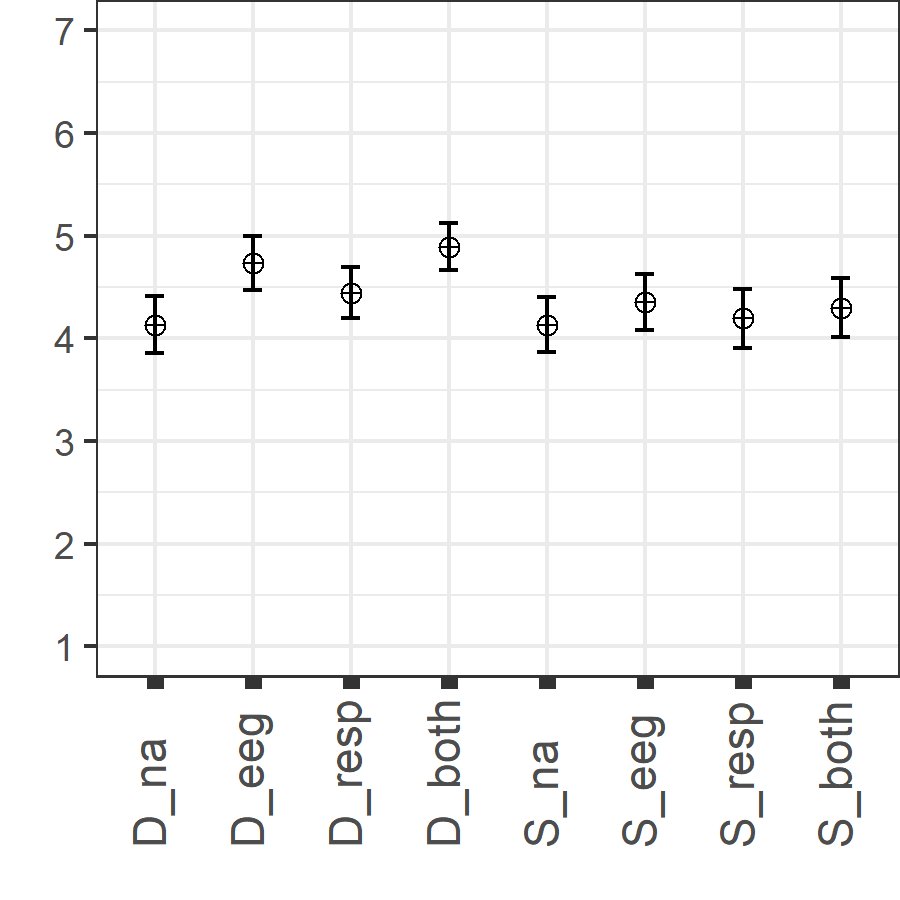
\includegraphics[width=0.5\textwidth]{images/EMP.png}
    \caption{\textcolor{blue}{Self-reported empathy scores with 95\% CI SE error bars across eight conditions of the study, showing the full scale of the instrument. D = dyadic condition, S = solo condition, na = no biofeedback, eeg = brainwave-based biofeedback, resp = breathing-based biofeedback, both = both biofeedbacks. Of note, self-reported empathy is higher in dyadic than solo condition when both forms of biofeedback are active, but not when only one form is active.}}
    \label{fig:batson}
\end{figure}


The core findings of the study can be summarized as follows:
\begin{enumerate}
\item Evoking empathy is easier when the VR space is shared and compassion meditation is directed at an active avatar
\item Social presence is stronger in dyadic conditions when the VR space is shared with another person
\item Mere sharing of space is not sufficient, empathy and social presence are increased only when the adaptations are on
\item Valence and dominance are higher in shared conditions, particularly when both adaptations are on
\item Biofeedbacks provide some degree of support valence related empathic accuracy in dyadic conditions
\item Only limited differences in physiological EDA or ECG synchrony was found between conditions, mainly, EDA synchrony was significant in solo condition without adaptations

\end{enumerate}

\subsection{Self-reports}

\begin{figure}
    % \noindent
    \centering
    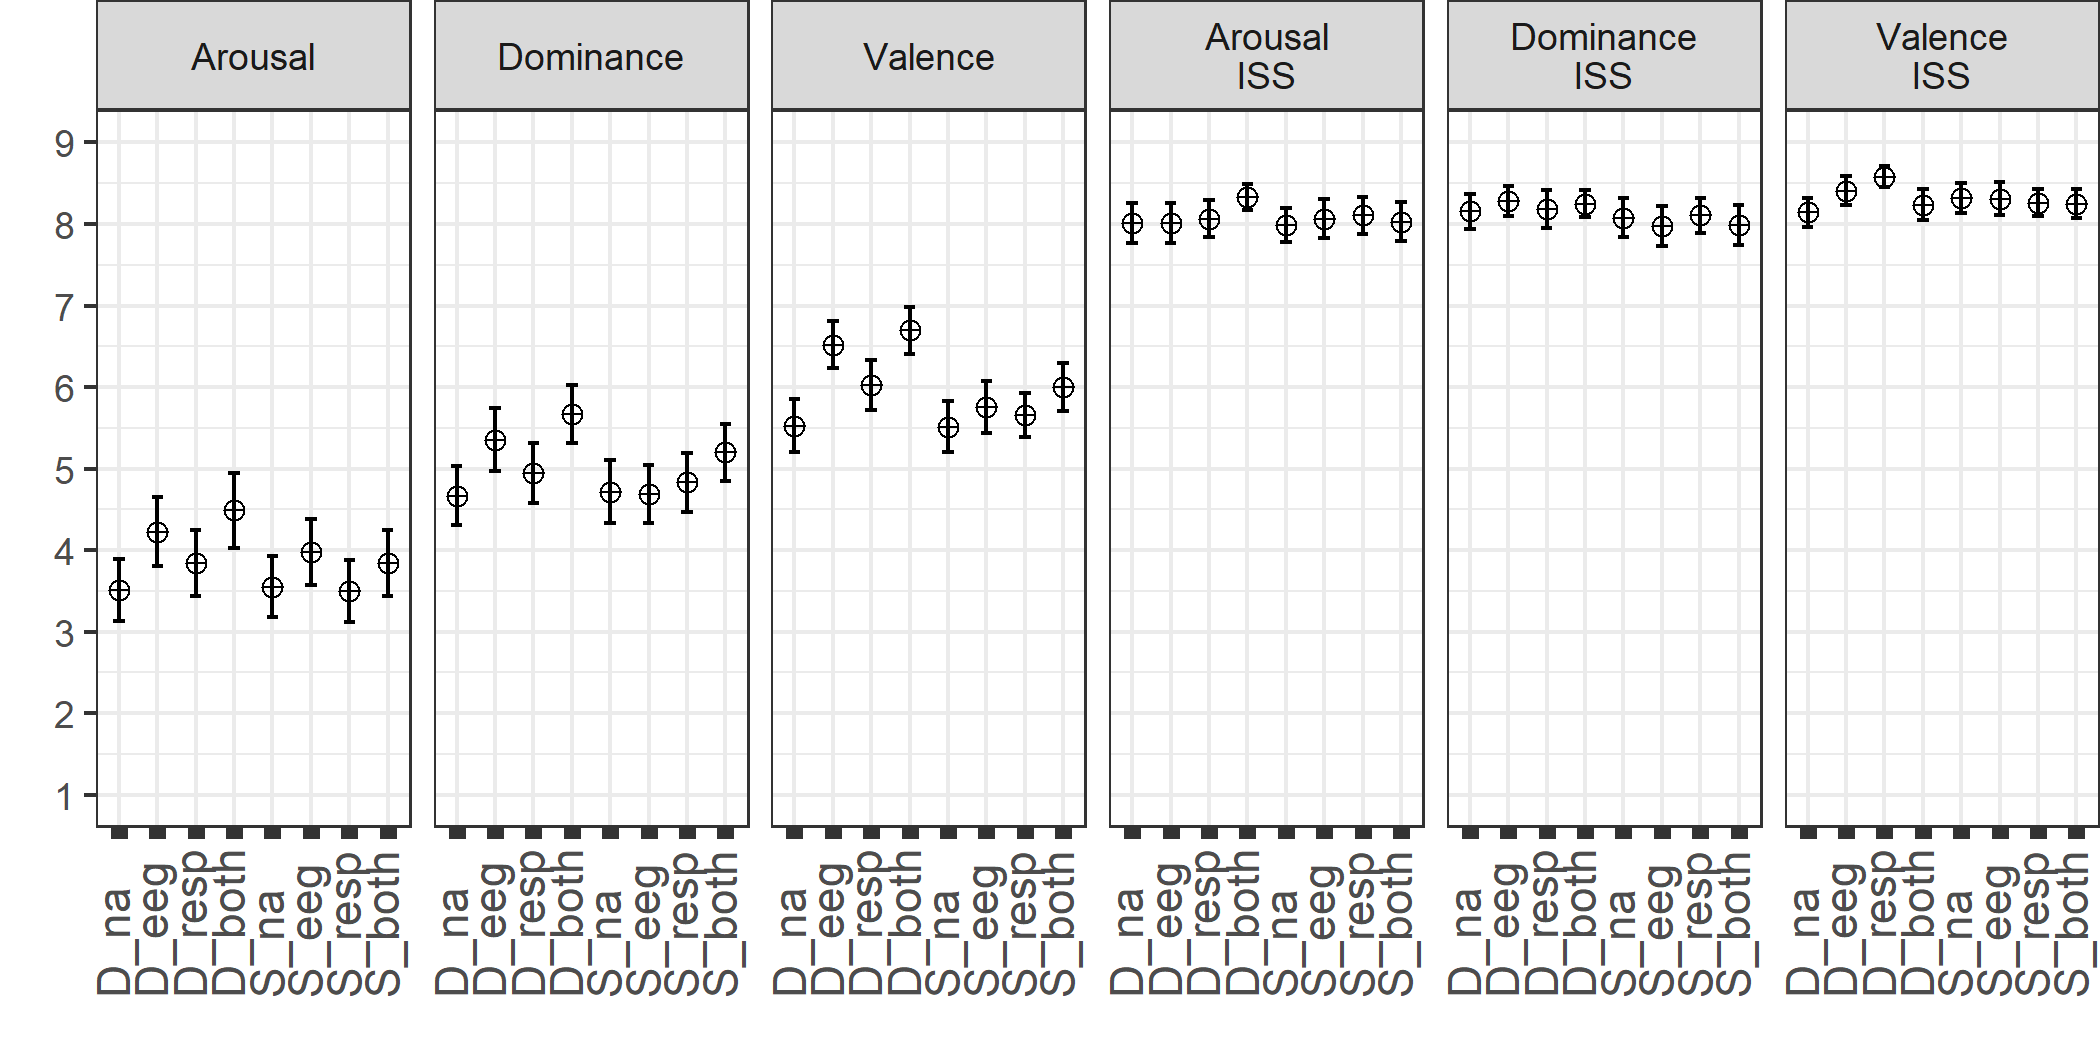
\includegraphics[width=\textwidth]{images/SAM.png}
    \caption{\textcolor{blue}{Self-Assessment Manakin scores for Arousal, Dominance, Valence, and their intersubjective symmetries (ISS) with 95\% CI SE error bars, across eight conditions of the study, showing the full scale of the instrument. D = dyadic condition, S = solo condition, na = no biofeedback, eeg = brainwave-based biofeedback, resp = breathing-based biofeedback, both = both biofeedbacks. While there is a trend for self-reports in dyadic with biofeedback conditions to be greater than solo conditions, the difference is clear only for Valence scores in `eeg' or `both' conditions.}}
    \label{fig:sam}
\end{figure}



The highest amount of self-reported empathy was evoked after the dyadic meditation sessions, where both the adaptations (EEG and respiration based) were active, and dyadic sessions with EEG and respiration adaptations the next highest (see Figure \ref{fig:batson}). There were no considerable differences between different adaptations in solo conditions, and clearly dyadic conditions with adaptations elicited more self-reported empathy. Almost identical pattern was found in self-reported emotional ratings: highest arousal, valence, and dominance was reported in dyadic conditions, particularly when both adaptations were on (Figure \ref{fig:sam}). In solo conditions, when both adaptations were on, higher valence and dominance were reported, otherwise the differences were small between solo conditions. Similarly, all social presence ratings --- Co-Presence, Affective Understanding, and Affective Interdependence --- were also higher in dyadic conditions when adaptations were on (Figure \ref{fig:sp}). The sense of social presence was strongest with both adaptations on, and EEG was more effective than respiration adaptation. Dyadic condition with no adaptation was rated similarly as solo conditions.

\begin{figure}
    % \noindent
    \centering
    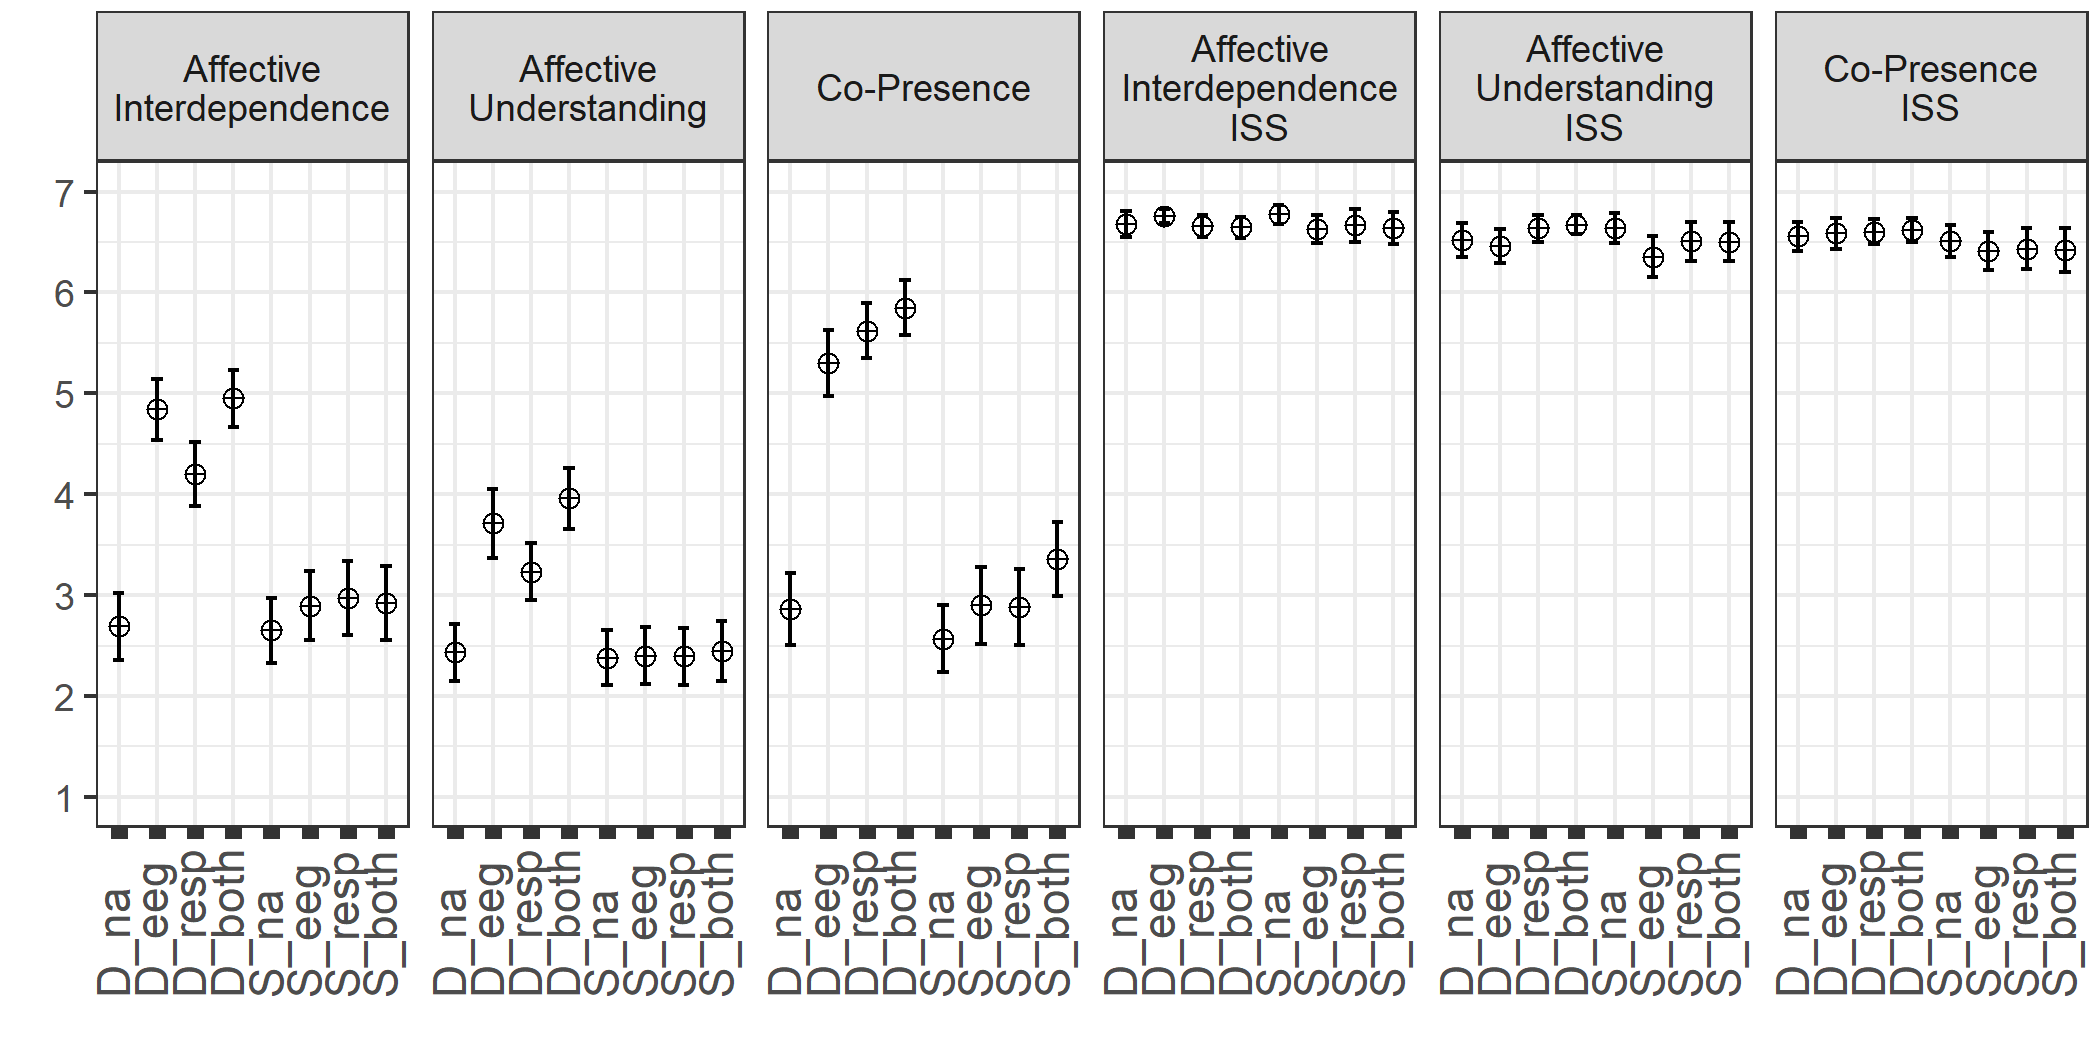
\includegraphics[width=\textwidth]{images/SP.png}
    \caption{\textcolor{blue}{Social Presence scores for Affective Interdependence, Affective Understanding, Co-Presence, and their intersubjective symmetries (ISS) with 95\% CI SE error bars, across eight conditions of the study, showing the full scale of the instrument. D = dyadic condition, S = solo condition, na = no biofeedback, eeg = brainwave-based biofeedback, resp = breathing-based biofeedback, both = both biofeedbacks. Note the clear the differences between dyadic with biofeedback vs. solo conditions.}}
    \label{fig:sp}
\end{figure}


Intersubjective symmetries of bi-directional self-reports were not largely affected by experimental manipulations, except in dyadic condition with respiration adaptations on, there was a higher degree of emotional symmetry on valence, that is, the empathic accuracy was higher. The symmetries were consistently higher on valence than on arousal or dominance. Social presence symmetries did vary across conditions, but affective interdependence symmetry were consistently higher than co-presence symmetry. 





\subsection{Physiological synchrony}
When conducting the permutation tests (Figure~\ref{fig:permutation}), it was observed that the amount of EDA synchrony within the dyad was mostly unaffected by solo vs. dyadic manipulation or the different types of biofeedbacks (D-both \textit{p} = .57, D-eeg \textit{p} = .74, D-resp \textit{p} = .64, D-na \textit{p} = .29, S-both \textit{p} = .54, S-eeg \textit{p} = .29, S-resp \textit{p} = .23, S-na \textit{p} < .005 \textcolor{blue}{ \& \textit{corrected p} < .05).} Thus, the only condition where significant synchrony was found was solo with no adaptations.

When examining HRV (heart rate variability) synchrony, the permutation tests show significant and marginal results in dyadic conditions with respiration adaptation and EEG adaptation, respectively (D-both \textit{p} = .71, D-eeg \textit{p} = .06 \textcolor{blue}{\& \textit{corrected p} = .42}, D-resp \textit{p} < .05 \textcolor{blue}{\& \textit{corrected p} = .4}, D-na \textit{p} = .95, S-both \textit{p} = .72, S-eeg \textit{p} = .98, S-resp \textit{p} = .96, S-na \textit{p} = .51).

\textcolor{blue}{After alpha corrections for multiple comparisons, only the solo with no biofeedback condition result for EDA synchrony remains significant at \textit{p} < 0.05.}

\begin{figure}[!ht]
    \centering
    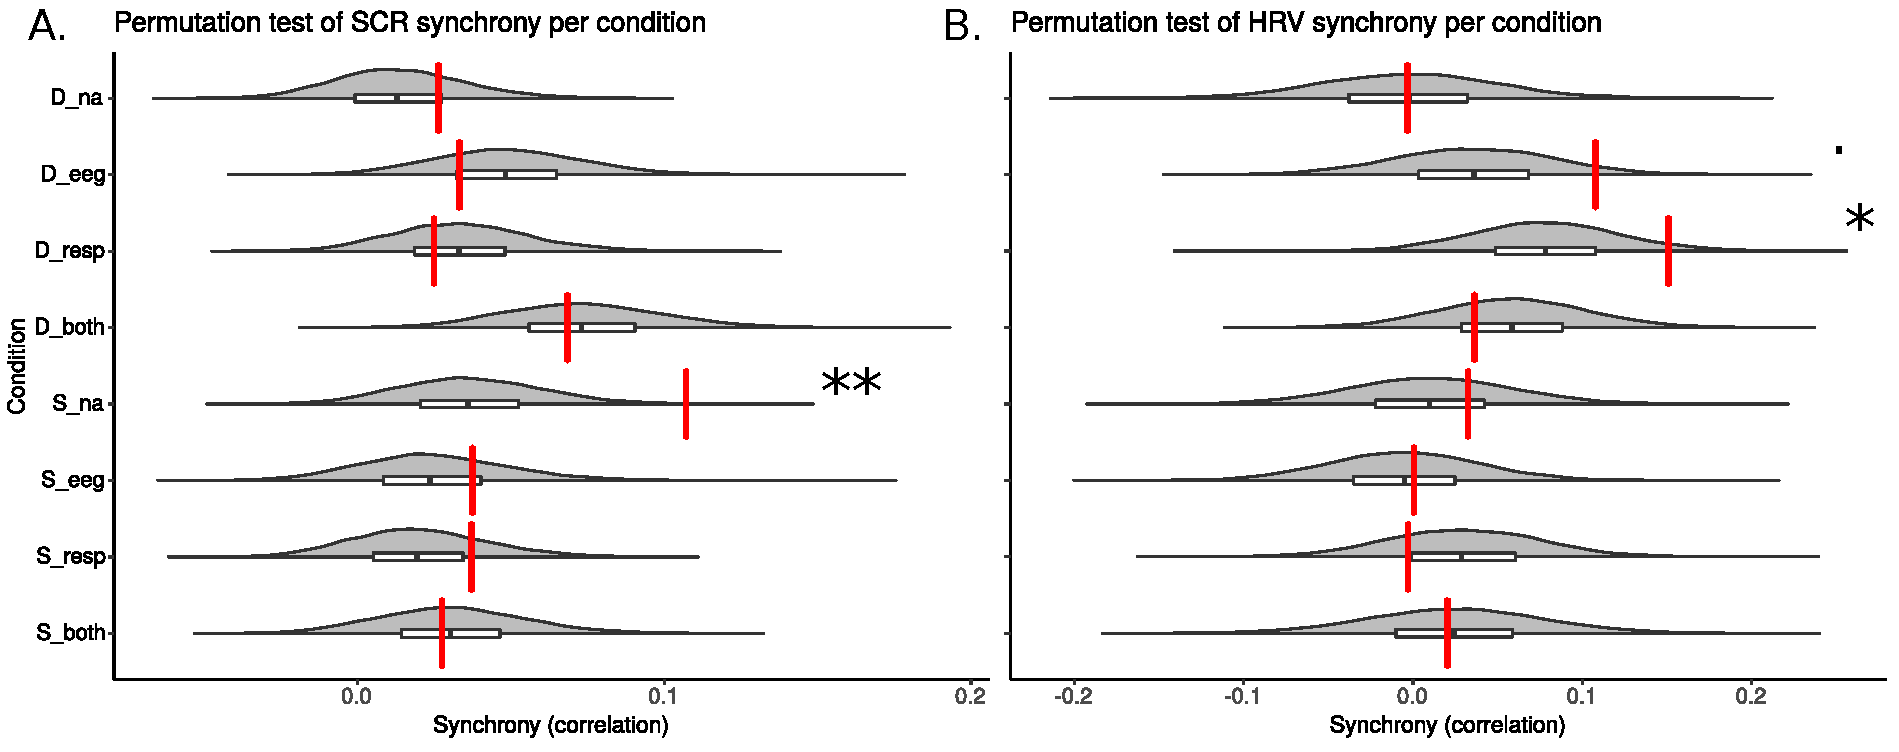
\includegraphics[width=\textwidth]{images/sync_SCR+HRV}
    \caption{Permutation tests of SCR (panel A) and HRV (panel B) synchrony across eight conditions of the study. Condition-wise half-violin plots represent the distributions of 10000 calculations of synchrony from randomly-permuted pseudo-dyads (boxplots drawn to aid inter-condition comparison); red vertical lines represent the observed synchrony in real dyads. The tests therefore show which conditions and physiological signals had a synchrony significantly outside the distribution generated by random pairings.\\ {\it p} < 0.1 `.', 0.05 `*', 0.01 `**'}
    \label{fig:permutation}
\end{figure}

\subsection{Self-reports and physiological synchrony}
Having observed the physiological synchrony results, we conducted an exploratory analysis of the relationship between participants' self-reports and the significant synchrony result, ie. solo without any adaptions for EDA synchrony. We constructed multiple regression models with all self-report items described above as independent variables, and synchrony as dependent variable.

EDA synchrony was significantly correlated only to Sex (\textit{p} < .05 \textcolor{blue}{ \& \textit{corrected p} = .2)}, close to significantly to Dominance ISS (\textit{p} = .09) and Affective Understanding ISS (\textit{p} < .09), but not Empathy (\textit{p} = .14), Arousal (\textit{p} = .58), Arousal ISS (\textit{p} = .36), Dominance (\textit{p} = .87), Valence (\textit{p} = .45), Valence ISS (\textit{p} = .18), Affective Interdependence (\textit{p} = .83), Affective Interdependence ISS (\textit{p} = .32), Affective Understanding (\textit{p} = .84), Co-Presence (\textit{p} = .49), Co-Presence ISS (\textit{p} = .18), Relationship Length (\textit{p} = .27), or Closeness (\textit{p} = .59). 

\textcolor{blue}{Notably, after alpha corrections for multiple comparisons, none of the relations between EDA synchrony and self-reports remain statistically significant.}



\section{Discussion}

Our experiment introduced a shared VR environment for compassion meditation with support from a variety of real-time biofeedbacks based on respiration and brainwaves. The ambitious experiment aimed to find: the effect of shared VR on empathy, emotions, social presence; the bi-directional assessments within the dyad when instructed to evoke compassionate and empathic feelings towards the other's VR avatar; and if these processes were supported by various forms of biofeedback. We also studied whether these manipulations increased physiological synchrony.

\textcolor{blue}{Answering the first research question \textit{"how are empathy and social presence affected by neurofeedback training with a partner in a VR meditation environment?"}}, the results paint a picture where empathy and social presence are easier to evoke when the VR space is shared with another person, and when it is supported by dyadic biofeedback. Also, to a limited degree, the biofeedbacks also support assessing the other persons emotional state. It is perhaps not entirely surprising that so called social emotions are more easily felt when directed at somebody who is present in the same virtual space, but the results do highlight the potential of shared VR spaces for joint meditation purposes, and showcase how empathic interactions are relevant in VR spaces even when isolated from any other form of interaction. The fact that empathy interaction is here experimentally controlled is itself a novel contribution.

The role of dyadic biofeedback was evident in the results, as the dyadic conditions with no feedback did not differ from the solo conditions, but adding respiration or EEG, or most efficiently both, adaptations did increase empathy, positive emotions, and social presence. This supports the initial idea that a biofeedback such as these provide socially utilizable affective information in otherwise scarce environment, and can be useful even if they do not aim at specific learning outcomes. These results showcase the potential for shared biofeedback meditations applications, and demonstrate that forms of augmented social meditation practices might be a fruitful direction for well-being oriented applications.

\textcolor{blue}{In relation to the second research question \textit{"how does dyadic synchrony biofeedback affect physiological synchrony within dyads?"}}, there was limited support for the idea that dyadic synchrony biofeedback would affect physiological synchrony itself. The respiration feedback condition had higher-than-random HRV synchrony, supported by permutation testing at {p} < 0.05, while EEG feedback saw a similar effect at {p} = 0.06 \textcolor{blue}{before any alpha corrections and only non-significant results after them.} The absolute synchrony value (i.e. average correlation) in these conditions was not high at just over 0.1, \textcolor{blue}{implying a very small effect size in general.}

There are several possible interpretations for the weak synchrony overall: the meditation period was so short that no discernible physiological synchrony between subjects formed; or the minimalistic VR environment and cutting off other channels of interaction for the participants inhibited the process through which physiological synchrony normally forms; possibly the biofeedbacks were too non-specific to interpret in a definitive manner, such that they did not affect physiological synchrony. It is plausible that the lack of results reflect all these factors, but without further extended studies it is impossible to interpret which of these was the most contributing factor.

However, the existing findings are intriguing. Notably, the biofeedbacks did not affect arousal in a synchronous manner, thus the single EDA synchrony result was found in solo condition with no biofeedback. Considering the nature of the environment and experimental setup, this most likely reflects how the experience of being alone in the environment without any biofeedback or interactivity is quite static and dominated by habituation to environmental factors like being in the experiment and sharing the same room. These factors are then shown in the EDA as similar patterns across participants, and consequently as higher degree of physiological synchrony even though it was not interactive or with additional information on the other person's physiological state. \textcolor{blue}{Notably, when examining the relation of this found synchrony effect and self-reports, no statistically significant results were found.} That the environmental stimuli in the DYNECOM VR do not induce synchronous SCRs is an unlooked-for positive outcome (from the design perspective), as it suggests that the environment is suitable for other forms of meditation also where disruptive VR features would only affect negatively the delicate attention processes trained while meditating. 

\textcolor{blue}{The pattern found when examining the uncorrected alpha levels for of HRV synchrony in dyadic respiration condition seems to reflect} the relation of breathing and cardiac activity. Considering that breathing is the chosen method in many meditation traditions to calm your inner state and that the respiration adaptation encourages the participants to synchronize the breathing rates, it is quite natural that increased HRV synchrony within dyad was observed, \textcolor{blue}{albeit barely. No strong inferences can be made based on the small effects of this study alone, but the observation hints at the future potential} of utilizing biofeedback to guide meditation practices in general, and the viability of joint meditation in shared VR with dyadic biofeedback. \textcolor{blue}{Continuing this line of speculative thinking oriented towards future work}, considering that EEG and respiration adaptations individually appeared to affect synchrony more than both of them together, it is possible that each reflect an attention-related effect. In other words, HRV synchrony is elicited more strongly by focusing on a single shared adaptation than a combination. Clinical neurofeedback applications typically prefer simpler single-channel setups for attention training, and here it might also be that a simple more explicit biofeedback is more effective at conveying social information on affective states in dyadic interactions.

\subsection{Limitations}
The experimental setup and the environment had some limitations that should be taken into account when interpreting the results and assessing the generalizability of the implications. Mainly, the limitations appeared as difficulties in making the virtual environment operate smoothly. For example, natural chest movements of the avatar, following respiration rhythm, had to be removed due to challenges with the network coding in Unity, and consequently only the more metaphoric respiration waves feedback was shown to the users. The color coding of EEG neurofeedback that was based on the idea of warm and cold colors, could have been counter-intuitive for those participants who interpreted them through a traffic lights metaphor (green = go, red = stop), though the misinterpretations were countered with explicit written instructions that clearly stated the meaning of the colors. Still, with biofeedback, intuitiveness is much preferred over mere rational understanding. \textcolor{blue}{No systematic data was collected how well the instructions were understood and if the visualizations were interpreted accordingly, but it is a possible source of error in the analysis but presumably covered by the sample size.} As is typical with extended VR sessions, some participants experienced some degree of VR sickness despite this element being taken into account beforehand in several ways in the test setup and in the design of the environment itself. However, in hindsight, the avatar to which the participant's focus was mostly directed at, incorporated too many fine details. Given the relatively low resolution of the system, this may have caused flickering that possibly contributed to some participants' reports of discomfort. 


\subsection{Conclusion}
In addition to illustrating the strong potential for augmenting compassion meditation in VR, and hence supporting the wellness and health benefits associated with meditation practice, these results suggest a broader impact. Dyadic neurofeedback pushes forward the possibilities of biofeedback, providing us with a novel method for feeding back information on low level core social processes such as presence, empathy and emotional connection. This idea can be utilized in a much wider spectrum of affective computing, ranging from virtual negotiation environments to therapy sessions. Indeed, the studies of physiological synchrony has its roots in patient-therapist interactions, and in many recent visions of the future of health technology VR has been highlighted as the new platform for therapy sessions. Biofeedback has potential in many forms of VR therapy, but dyadic synchrony feedback is naturally particularly useful for forms of therapy with a therapist-patient setting. With this ground-breaking experiment, we hope to encourage a wide range of experimental studies delving into the very nature of dyadic synchrony and feedback, and hope to see innovative prototypes utilizing them in various technological setups. Additionally, DYNECOM utilized respiration and EEG; other biosignals -- particularly those that are more easily deployed as wearable consumer grade devices, such as heart rate or skin conductance based measures -- should also be examined and their usefulness in this use case mapped out. 



%  \section{Introduction}
% ACM's consolidated article template, introduced in 2017, provides a consistent \LaTeX\ style for use across ACM publications, and incorporates accessibility and metadata-extraction functionality necessary for future Digital Library endeavors. Numerous ACM and SIG-specific \LaTeX\ templates have been examined, and their unique features incorporated into this single new template.

% If you are new to publishing with ACM, this document is a valuable guide to the process of preparing your work for publication. If you have published with ACM before, this document provides insight and instruction into more recent changes to the article template.

% The ``\verb|acmart|'' document class can be used to prepare articles for any ACM publication --- conference or journal, and for any stage of publication, from review to final ``camera-ready'' copy, to the author's own version, with {\it very} few changes to the source.

% \section{Template Overview}
% As noted in the introduction, the ``\verb|acmart|'' document class can be used to prepare many different kinds of documentation --- a double-blind initial submission of a full-length technical paper, a two-page SIGGRAPH Emerging Technologies abstract, a ``camera-ready'' journal article, a SIGCHI Extended Abstract, and more --- all by selecting the appropriate {\it template style} and {\it template parameters}.

% This document will explain the major features of the document class. For further information, the {\it \LaTeX\ User's Guide} is available from \url{https://www.acm.org/publications/proceedings-template}.

% \subsection{Template Styles}

% The primary parameter given to the ``\verb|acmart|'' document class is the {\it template style} which corresponds to the kind of publication or SIG publishing the work. This parameter is enclosed in square brackets and is a part of the {\verb|documentclass|} command:
% \begin{verbatim}
  % \documentclass[STYLE]{acmart}
% \end{verbatim}

%Journals use one of three template styles. All but three ACM journals use the {\verb|acmsmall|} template style:
%\begin{itemize}
%\item {\verb|acmsmall|}: The default journal template style.
%\item {\verb|acmlarge|}: Used by JOCCH and TAP.
%\item {\verb|acmtog|}: Used by TOG.
%\end{itemize}

%he majority of conference proceedings documentation will use the {\verb|acmconf|} template style.
%\begin{itemize}
%\item {\verb|acmconf|}: The default proceedings template style.
%\item{\verb|sigchi|}: Used for SIGCHI conference articles.
%\item{\verb|sigchi-a|}: Used for SIGCHI ``Extended Abstract'' articles.
%\item{\verb|sigplan|}: Used for SIGPLAN conference articles.
%\end{itemize}

%\subsection{Template Parameters}

%In addition to specifying the {\it template style} to be used in formatting your work, there are a number of {\it template parameters} which modify some part of the applied template style. A complete list of these parameters can be found in the {\it \LaTeX\ User's Guide.}

%Frequently-used parameters, or combinations of parameters, include:
%\begin{itemize}
%\item {\verb|anonymous,review|}: Suitable for a ``double-blind'' conference submission. Anonymizes the work and includes line numbers. Use with the \verb|\acmSubmissionID| command to print the submission's unique ID on each page of the work.
%\item{\verb|authorversion|}: Produces a version of the work suitable for posting by the author.
%\item{\verb|screen|}: Produces colored hyperlinks.
%\end{itemize}

%This document uses the following string as the first command in the source file: \verb|\documentclass[sigconf,screen]{acmart}|.

%\section{Modifications}

%Modifying the template --- including but not limited to: adjusting margins, typeface sizes, line spacing, paragraph and list definitions, and the use of the \verb|\vspace| command to manually adjust the vertical spacing between elements of your work --- is not allowed.

%{\bf Your document will be returned to you for revision if modifications are discovered.}

%\section{Typefaces}

%The ``\verb|acmart|'' document class requires the use of the ``Libertine'' typeface family. Your \TeX\ installation should include this set of packages. Please do not substitute other typefaces. The ``\verb|lmodern|'' and ``\verb|ltimes|'' packages should not be used, as they will override the built-in typeface families.

%\section{Title Information}

%The title of your work should use capital letters appropriately - \url{https://capitalizemytitle.com/} has useful rules for capitalization. Use the {\verb|title|} command to define the title of your work. If your work has a subtitle, define it with the {\verb|subtitle|} command.
%Do not insert line breaks in your title.

%If your title is lengthy, you must define a short version to be used in the page headers, to prevent overlapping text. The \verb|title| command has a ``short title'' parameter:
%\begin{verbatim}
%  \title[short title]{full title}
%\end{verbatim}

% \section{Authors and Affiliations}

% Each author must be defined separately for accurate metadata identification. Multiple authors may share one affiliation. Authors' names should not be abbreviated; use full first names wherever possible. Include authors' e-mail addresses whenever possible.

% Grouping authors' names or e-mail addresses, or providing an ``e-mail alias,'' as shown below, is not acceptable:
% \begin{verbatim}
  % \author{Brooke Aster, David Mehldau}
  % \email{dave,judy,steve@university.edu}
  % \email{firstname.lastname@phillips.org}
% \end{verbatim}

% The \verb|authornote| and \verb|authornotemark| commands allow a note to apply to multiple authors --- for example, if the first two authors of an article contributed equally to the work.

% If your author list is lengthy, you must define a shortened version of the list of authors to be used in the page headers, to prevent overlapping text. The following command should be placed just after the last \verb|\author{}| definition:
% \begin{verbatim}
  %\renewcommand{\shortauthors}{McCartney, et al.}
% \end{verbatim}
% Omitting this command will force the use of a concatenated list of all of the authors' names, which may result in overlapping text in the page headers.

% The article template's documentation, available at  \url{https://www.acm.org/publications/proceedings-template}, has a complete explanation of these commands and tips for their effective use.

% \section{Rights Information}

% Authors of any work published by ACM will need to complete a rights form. Depending on the kind of work, and the rights management choice made by the author, this may be copyright transfer, permission, license, or an OA (open access) agreement.

%Regardless of the rights management choice, the author will receive a copy of the completed rights form once it has been submitted. This form contains \LaTeX\ commands that must be copied into the source document. When the document source is compiled, these commands and their parameters add formatted text to several areas of the final document:
%\begin{itemize}
%\item the ``ACM Reference Format'' text on the first page.
%\item the ``rights management'' text on the first page.
%\item the conference information in the page header(s).
%\end{itemize}

% Rights information is unique to the work; if you are preparing several works for an event, make sure to use the correct set of commands with each of the works.

% \section{CCS Concepts and User-Defined Keywords}

% Two elements of the ``acmart'' document class provide powerful taxonomic tools for you to help readers find your work in an online search.

% The ACM Computing Classification System --- \url{https://www.acm.org/publications/class-2012} --- is a set of classifiers and concepts that describe the computing discipline. Authors can select entries from this classification system, via \url{https://dl.acm.org/ccs/ccs.cfm}, and generate the commands to be included in the \LaTeX\ source.

% User-defined keywords are a comma-separated list of words and phrases of the authors' choosing, providing a more flexible way of describing the research being presented.

% CCS concepts and user-defined keywords are required for all short- and full-length articles, and optional for two-page abstracts.

% \section{Sectioning Commands}

% Your work should use standard \LaTeX\ sectioning commands: \verb|section|, \verb|subsection|, \verb|subsubsection|, and \verb|paragraph|. They should be numbered; do not remove the numbering from the commands.

% Simulating a sectioning command by setting the first word or words of a paragraph in boldface or italicized text is {\bf not allowed.}

% \section{Tables}

% The ``\verb|acmart|'' document class includes the ``\verb|booktabs|'' package --- \url{https://ctan.org/pkg/booktabs} --- for preparing high-quality tables.

% Table captions are placed {\it above} the table.

% Because tables cannot be split across pages, the best placement for them is typically the top of the page nearest their initial cite.  To ensure this proper ``floating'' placement of tables, use the environment \textbf{table} to enclose the table's contents and the table caption.  The contents of the table itself must go in the \textbf{tabular} environment, to be aligned properly in rows and columns, with the desired horizontal and vertical rules.  Again, detailed instructions on \textbf{tabular} material are found in the \textit{\LaTeX\ User's Guide}.

% Immediately following this sentence is the point at which Table~\ref{tab:freq} is included in the input file; compare the placement of the table here with the table in the printed output of this document.

%\begin{table}
 % \caption{Frequency of Special Characters}
 % \label{tab:freq}
 % \begin{tabular}{ccl}
  %  \toprule
   % Non-English or Math&Frequency&Comments\\
%    \midrule
 %   \O & 1 in 1,000& For Swedish names\\
  %  $\pi$ & 1 in 5& Common in math\\
   % \$ & 4 in 5 & Used in business\\
%    $\Psi^2_1$ & 1 in 40,000& Unexplained usage\\
 % \bottomrule
% \end{tabular}
% \end{table}

% To set a wider table, which takes up the whole width of the page's live area, use the environment \textbf{table*} to enclose the table's contents and the table caption.  As with a single-column table, this wide table will ``float'' to a location deemed more desirable. Immediately following this sentence is the point at which Table~\ref{tab:commands} is included in the input file; again, it is instructive to compare the placement of the table here with the table in the printed output of this document.

% \begin{table*}
 % \caption{Some Typical Commands}
 % \label{tab:commands}
 % \begin{tabular}{ccl}
 %   \toprule
 %   Command &A Number & Comments\\
 %   \midrule
 %   \texttt{{\char'134}author} & 100& Author \\
 %   \texttt{{\char'134}table}& 300 & For tables\\
 %   \texttt{{\char'134}table*}& 400& For wider tables\\
 %   \bottomrule
 % \end{tabular}
% \end{table*}


% \section{Figures}

% The ``\verb|figure|'' environment should be used for figures. One or more images can be placed within a figure. If your figure contains third-party material, you must clearly identify it as such, as shown in the example below.
% \begin{figure}[h]
%  \centering
%  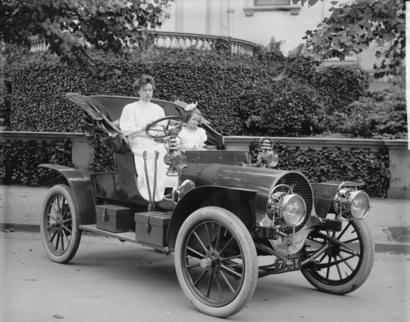
\includegraphics[width=\linewidth]{sample-franklin}
%  \caption{1907 Franklin Model D roadster. Photograph by Harris \& Ewing, Inc. [Public domain], via Wikimedia Commons. (\url{https://goo.gl/VLCRBB}).}
%  \Description{The 1907 Franklin Model D roadster.}
%\end{figure}

% Your figures should contain a caption which describes the figure to the reader. Figure captions go below the figure. Your figures should {\bf also} include a description suitable for screen readers, to assist the visually-challenged to better understand your work.

% Figure captions are placed {\it below} the figure.

%\subsection{The ``Teaser Figure''}

%A ``teaser figure'' is an image, or set of images in one figure, that are placed after all author and affiliation information, and before the body of the article, spanning the page. If you wish to have such a figure in your article, place the command immediately before the \verb|\maketitle| command:
%\begin{verbatim}
%  \begin{teaserfigure}
%    \includegraphics[width=\textwidth]{sampleteaser}
%    \caption{figure caption}
%    \Description{figure description}
%  \end{teaserfigure}
%\end{verbatim}

% \section{Citations and Bibliographies}

%The use of \BibTeX\ for the preparation and formatting of one's references is strongly recommended. Authors' names should be complete --- use full first names (``Donald E. Knuth'') not initials (``D. E. Knuth'') --- and the salient identifying features of a reference should be included: title, year, volume, number, pages, article DOI, etc.

%The bibliography is included in your source document with these two commands, placed just before the %\verb|\end{document}| command:
%\begin{verbatim}
%  \bibliographystyle{ACM-Reference-Format}
%  \bibliography{bibfile}
% \end{verbatim}
%where ``\verb|bibfile|'' is the name, without the ``\verb|.bib|'' suffix, of the \BibTeX\ file.

%Citations and references are numbered by default. A small number of ACM publications have citations and references formatted in the ``author year'' style; for these exceptions, please include this command in the {\bf preamble} (before ``\verb|\begin{document}|'') of your \LaTeX\ source:
%\begin{verbatim}
%  \citestyle{acmauthoryear}
% \end{verbatim}

%Some examples.  A paginated journal article \cite{Abril07}, an enumerated journal article \cite{Cohen07}, a reference to an entire issue \cite{JCohen96}, a monograph (whole book) \cite{Kosiur01}, a monograph/whole book in a series (see 2a in spec. document)
%\cite{Harel79}, a divisible-book such as an anthology or compilation \cite{Editor00} followed by the same example, however we only output the series if the volume number is given \cite{Editor00a} (so Editor00a's series should NOT be present since it has no vol. no.),
%a chapter in a divisible book \cite{Spector90}, a chapter in a divisible book in a series \cite{Douglass98}, a multi-volume work as book \cite{Knuth97}, an article in a proceedings (of a conference, symposium, workshop for example) (paginated proceedings article) \cite{Andler79}, a proceedings article with all possible elements \cite{Smith10}, an example of an enumerated proceedings article \cite{VanGundy07}, an informally published work \cite{Harel78}, a doctoral dissertation \cite{Clarkson85}, a master's thesis: \cite{anisi03}, an online document / world wide web resource \cite{Thornburg01, Ablamowicz07, Poker06}, a video game (Case 1) \cite{Obama08} and (Case 2) \cite{Novak03} and \cite{Lee05} and (Case 3) a patent \cite{JoeScientist001}, work accepted for publication \cite{rous08}, 'YYYYb'-test for prolific author \cite{SaeediMEJ10} and \cite{SaeediJETC10}. Other cites might contain 'duplicate' DOI and URLs (some SIAM articles) \cite{Kirschmer:2010:AEI:1958016.1958018}. Boris / Barbara Beeton: multi-volume works as books \cite{MR781536} and \cite{MR781537}. A couple of citations with DOIs: \cite{2004:ITE:1009386.1010128,Kirschmer:2010:AEI:1958016.1958018}. Online citations: \cite{TUGInstmem, Thornburg01, CTANacmart}.

%\section{Acknowledgments}

%Identification of funding sources and other support, and thanks to individuals and groups that assisted in the research and the preparation of the work should be included in an acknowledgment section, which is placed just before the reference section in your document.

%This section has a special environment:
%\begin{verbatim}
%  \begin{acks}
%  ...
%  \end{acks}
%\end{verbatim}
%so that the information contained therein can be more easily collected during the article metadata extraction phase, and to ensure consistency in the spelling of the section heading.

%Authors should not prepare this section as a numbered or unnumbered {\verb|\section|}; please use the ``{\verb|acks|}'' environment.

%\section{Appendices}

%If your work needs an appendix, add it before the ``\verb|\end{document}|'' command at the conclusion of your source document.

%Start the appendix with the ``\verb|appendix|'' command:
%\begin{verbatim}
%  \appendix
%\end{verbatim}
%and note that in the appendix, sections are lettered, not numbered. This document has two appendices, demonstrating the section and subsection identification method.

%\section{SIGCHI Extended Abstracts}

%The ``\verb|sigchi-a|'' template style (available only in \LaTeX\ and not in Word) produces a landscape-orientation formatted article, with a wide left margin. Three environments are available for use with the ``\verb|sigchi-a|'' template style, and produce formatted output in the margin:
%\begin{itemize}
%\item {\verb|sidebar|}:  Place formatted text in the margin.
%\item {\verb|marginfigure|}: Place a figure in the margin.
%\item {\verb|margintable|}: Place a table in the margin.
%\end{itemize}

%
% The acknowledgments section is defined using the "acks" environment (and NOT an unnumbered section). This ensures
% the proper identification of the section in the article metadata, and the consistent spelling of the heading.
\begin{acks}
We would like to thank Antti Ruonala, Janne Timonen, and Kristiina Mannermaa for their efforts in technical development of environment, data collection, and in contributing to earlier versions of the manuscript. The work was supported by The Academy of Finland (project EMOEMP: 305576 and 305577). 

\end{acks}

%
% The next two lines define the bibliography style to be used, and the bibliography file.
\bibliographystyle{ACM-Reference-Format}
\bibliography{refs}

%
% If your work has an appendix, this is the place to put it.
%\appendix

%\section{Research Methods}

%\subsection{Part One}

%Lorem ipsum dolor sit amet, consectetur adipiscing elit. Morbi malesuada, quam in pulvinar varius, metus nunc fermentum urna, id sollicitudin purus odio sit amet enim. Aliquam ullamcorper eu ipsum vel mollis. Curabitur quis dictum nisl. Phasellus vel semper risus, et lacinia dolor. Integer ultricies commodo sem nec semper.

%\subsection{Part Two}

%Etiam commodo feugiat nisl pulvinar pellentesque. Etiam auctor sodales ligula, non varius nibh pulvinar semper. Suspendisse nec lectus non ipsum convallis congue hendrerit vitae sapien. Donec at laoreet eros. Vivamus non purus placerat, scelerisque diam eu, cursus ante. Etiam aliquam tortor auctor efficitur mattis.

%\section{Online Resources}

%Nam id fermentum dui. Suspendisse sagittis tortor a nulla mollis, in pulvinar ex pretium. Sed interdum orci quis metus euismod, et sagittis enim maximus. Vestibulum gravida massa ut felis suscipit congue. Quisque mattis elit a risus ultrices commodo venenatis eget dui. Etiam sagittis eleifend elementum.

% Nam interdum magna at lectus dignissim, ac dignissim lorem rhoncus. Maecenas eu arcu ac neque placerat aliquam. Nunc pulvinar massa et mattis lacinia.

\end{document}